\section{Research-Continuity Studies}
\label{app:architecture-ablations}
\subsection{Task-Level Knowledge/Skill Comparison}
The four K/S configurations comprise 44 task cells evaluated under strictly identical resource-budget ceilings. Each cell is evaluated against the complete task protocol, and the recorded selection and acceptance determine task completion. All incomplete runs terminate upon budget exhaustion. Table~\ref{tab:abc-comparison} gives the task outcomes; Appendix~\ref{app:cross-model-profile} reports aggregate workload.

\subsection{Reporter Decision Replay}
Six matched checkpoints are replayed with the saved Reporter interpretation withheld or included, producing twelve Main Agent sessions. Each pair uses the same task, candidate, and evidence snapshot. An independent model reviews anonymized proposed decisions on five dimensions scored from 0 to 4: physical interpretation, evidence consistency, limitation recognition, research actionability, and decision quality.

The equal-weight mean is 3.433 with Reporter OFF and 3.733 with Reporter ON, with two improvements and four ties across the six pairs. Unsupported conclusions occur twice in OFF and zero times in ON. Figure~\ref{fig:research-continuity}A shows the paired scores.

\subsection{Hierarchical Context Replay}
Flat delivery supplies the checkpoint corpus; hierarchical delivery supplies an L0 brief and access to supporting records. At the load-diagnosis checkpoint, accepted-request input is 675,802 tokens for Flat and 78,785 for hierarchical delivery, with decision scores of 4.0 and 3.8. At the parameter-tradeoff checkpoint, cumulative accepted-request input is 877,197 and 174,298 tokens, with decision scores of 3.4 and 3.6 and key-evidence coverage of 5/5 and 3/5. The reductions are 88.34\% and 80.13\%, respectively (Fig.~\ref{fig:research-continuity}B).
\begin{figure}[!htbp]
\centering
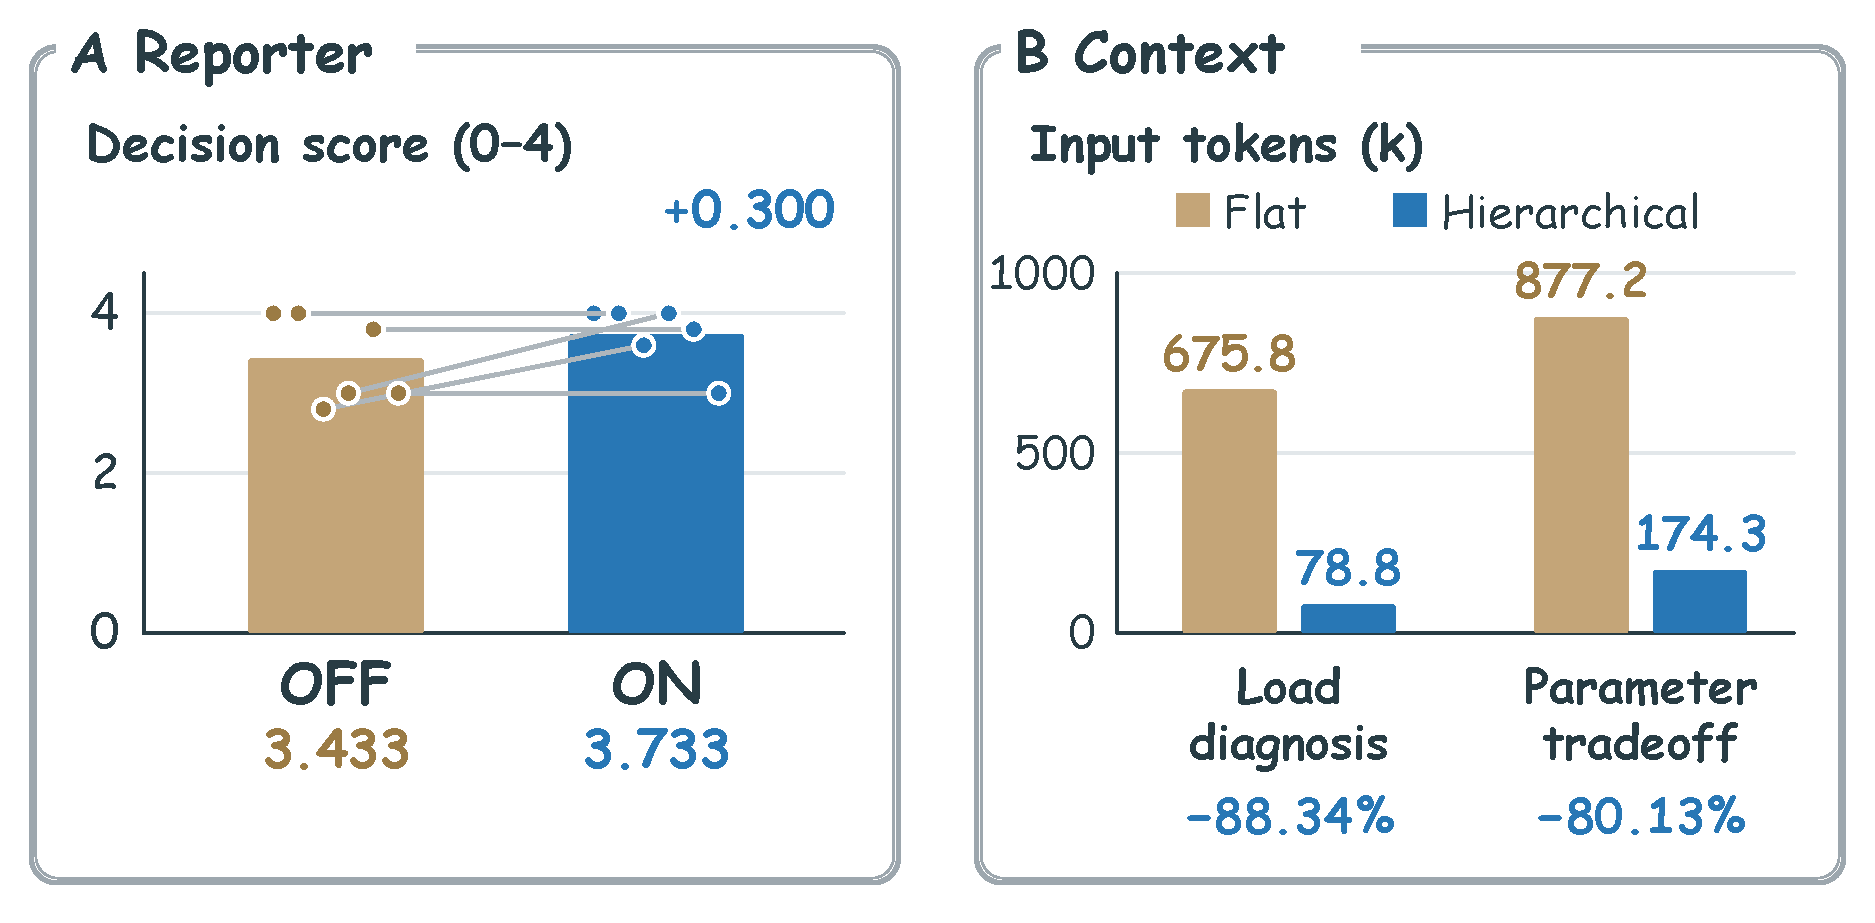
\includegraphics[width=\columnwidth]{figures/fig05_research_continuity.pdf}
\caption{Reporter and hierarchical-context comparisons.
(A) Mean five-dimension blind-review scores across six
matched decisions: two improve, four remain unchanged,
and unsupported claims decrease from two to zero.
(B) Provider-reported input tokens under flat and
hierarchical context at the load-diagnosis and
parameter-tradeoff checkpoints.}
\label{fig:research-continuity}
\end{figure}

